\documentclass[handout]{beamer}
\usepackage{textpos}
\usepackage{listings}


\usepackage{xcolor}
\definecolor{mygreen}{rgb}{0,0.6,0}
\definecolor{mygray}{rgb}{0.5,0.5,0.5}

\lstset{language=C++,
           basicstyle=\ttfamily\scriptsize,
           keywordstyle=\color{blue}\ttfamily,
           stringstyle=\color{red}\ttfamily,
           commentstyle=\color{mygreen}\ttfamily,
          breaklines=true,
          captionpos=b,
          numbers=left,
          numbersep=5pt,
          numberstyle=\tiny\color{mygray},
          rulecolor=\color{black},
          xleftmargin=\parindent,
          frame=single,
          backgroundcolor=\color{white}
}

% \usepackage{beamerthemesplit} // Activate for custom appearance
%\usecolortheme{whale}
\setbeamercolor{normal text}{fg=black,bg=white}
\definecolor{beamer@blendedblue}{rgb}{0,0,0}
\setbeamercolor{structure}{fg=beamer@blendedblue}


\title{Introduction to Massively Parallel Computing (with CUDA)}
\author{
	\includegraphics[width=3cm]{../media/logo/NVLogo_2D.eps}
	\vspace{0.75cm}
	\\}
\date{\today}

\begin{document}

\frame{\titlepage}

%\section[Outline]{}
\begin{frame}{Outline}
\tableofcontents
\end{frame}


\addtobeamertemplate{frametitle}{}{%
\begin{textblock*}{200mm}(.75\textwidth,-0.35cm)
\includegraphics[width=3cm]{../media/logo/NVLogo_2D_H.eps}
\end{textblock*}}

\addtobeamertemplate{navigation symbols}{}{%
    \usebeamerfont{footline}%
    \usebeamercolor[fg]{footline}%
    \hspace{1em}%
    \insertframenumber/\inserttotalframenumber
}

%\section{Introduction}
%\subsection{Overview of the Beamer Class}

%\frame
%{
 %\frametitle{What is CUDA?}
%
%  \begin{itemize}
%  \item<1-> Normal LaTeX class.
%  \item<2-> Easy overlays.
%  \item<3-> No external programs needed.      
%  \end{itemize}
%}

\begin{frame}{What is CUDA?}
\section{What is CUDA?}
\emph{CUDA is a parallel computing platform and application programming interface (API) model created by NVIDIA. It allows software developers and software engineers to use a CUDA-enabled graphics processing unit (GPU) for general purpose processing - an approach known as GPGPU [computing].\footnote{Wikipedia}}

\end{frame}

\begin{frame}{What is CUDA?}
\emph{CUDA is a parallel computing platform and programming model that makes using a GPU for general purpose computing simple and elegant. The developer still programs in the familiar C, C++, Fortran, or an ever expanding list of supported languages, and incorporates extensions of these languages in the form of a few basic keywords}.\footnote{blogs.nvidia.com}
\end{frame}

\section{Heterogeneous Architecture}  
\begin{frame}{Heterogeneous Architecture}
\begin{itemize}
  \item<1-> A GPU is not a standalone platform but rather a co-processor to the CPU
  \item<2-> GPUs must operate in conjunction with CPU-based host through a PCI-Express bus
  \item<3-> In GPU computing terms, the CPU is called the \emph{host} and the GPU is called the \emph{device}
  \item<4->Heterogeneous applications include both 
  	\begin{itemize}
  		\item {Host code (C, C++) which runs on the CPU}
		\item {Device code (C-lang \emph{Kernels}) which runs on the GPU}
  	\end{itemize}
  \item<5->The CPU code is responsible for managing the environment, code, and data for the device before loading compute-intensive tasks on the device	
\end{itemize}
\end{frame}

\begin{frame}{Heterogeneous Architecture}
\begin{itemize}
\itemsep1em
	\item<1-> Since the GPU is physically separate from the CPU, it can most generically be referred to as a \emph{hardware accelerator}
	\item<2->The general idea is that GPUs are used only to accelerate portions of application code which exhibit rich amounts of data parallelism (i.e. linear algebra, image proc, FFTs, etc)
\end{itemize}
\end{frame}

\section{CPU/GPU Design Considerations}
\begin{frame}{CPU/GPU Design Considerations}
\begin{itemize}
\setbeamercovered{transparent}
	\item<1->GPU computing is not meant to replace CPU computing.  Each approach has advantages for certain kinds of applications. 
	\item<2->Multicore microprocessors, like Intel Core i7, are optimized for for sequential instruction execution performance. These multicore CPU designs make use of sophisticated control logic and very large shared caches to allow instructions from a single thread of execution to execute in parallel or even out of sequence while maintaining the appearance of sequential execution
	\item<3->On the other hand, the massively parallel streaming processor design of GPUs utilize many threads of execution over huge number of smaller cores. For example, GeForce TitanX has 3072 cores (24 SM $\times$ 128 cores/SM).
\end{itemize}
\end{frame}

\begin{frame}{CPU/GPU Design Considerations}
 \begin{figure}[ht]
 \label{fig:cpu_gpu_arch}
    	\begin{center}
        		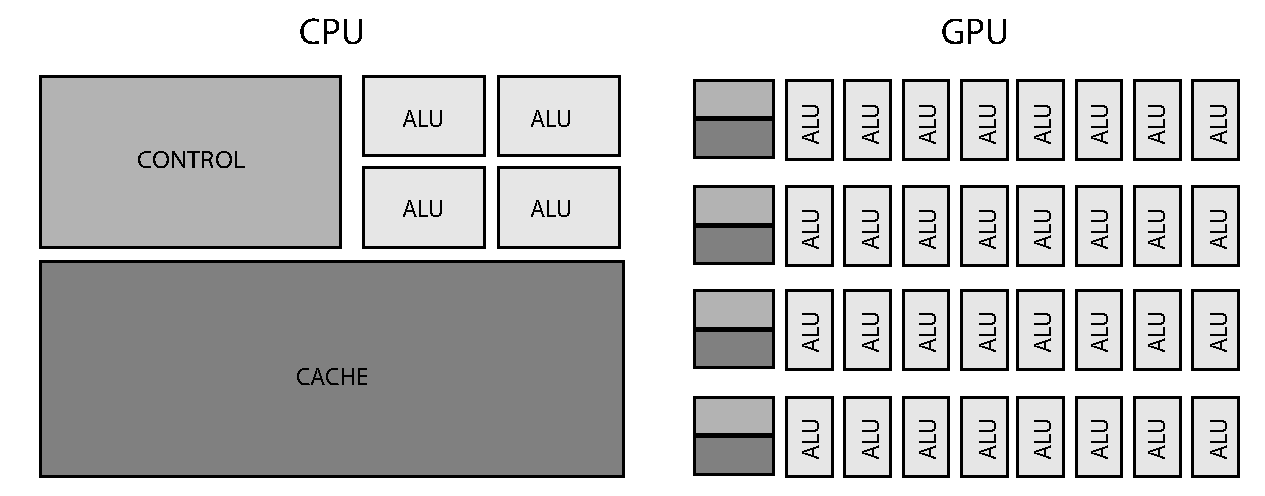
\includegraphics[width=10cm]{../media/gpu_cpu_arch.pdf}
      \end{center}
 	\caption{CPUs and GPUs have fundamentally different design philosophies}
    \end{figure}
\end{frame}

\begin{frame}{CPU/GPU Design Considerations}
\begin{itemize}
\setbeamercovered{transparent}
	\item<1->The design philosophy of the GPU was historically shaped by the fast-growing video game industry that exerted tremendous economic pressure for the ability to perform massive number of floating-point calculations per video frame.
	\item<2->This demand motivated GPU architects to look for ways to maximize the chip area and power budget dedicated to floating-point arithmetic. 
	\item<3->The prevailing solution is to optimize for the execution throughput of massive numbers of threads by allowing piplined memory channels and arithmetic ops to have long latency.
	\item<4->This design minimizes chip area and power of both memory access hardware and ALUs allowing for more of each on chip thus increasing total execution throughput.
\end{itemize}
\end{frame}

\begin{frame}{CPU/GPU Design Considerations}
\begin{itemize}
	\setbeamercovered{transparent}
	\item<1->This GPU chip design style is commonly referred to as \emph{throughput-oriented} design since it strives to maximize the total execution throughput of a large number of threads.
	\item<2-> The CPU chip design, on the other hand, strives to minimize the execution latency of a single thread and is often referred to as \emph{latency-oriented} design.
	\item<3->Think of these design contrasts as the difference between local versus global optimization strategies.
\end{itemize}
\end{frame}

\begin{frame}{CPU/GPU Design Considerations}
\begin{itemize}
	\item<1->OK, I get it $\ldots$  but why is throughput-oriented effective on GPUs?
	\item<2->For a typical CPU scenario, each thread of execution is a different application (e.g. Microsoft Office, Netflix, Angry Birds).  That is, multiple concurrent threads executing independent applications.
	\item<3->However, on a GPU all threads are working in parallel to execute a single kernel/task (e.g. multiply these two matrices, white balance this image, etc). 
	\item<4->Therefore, the throughput-oriented kernel execution says something like ``\emph{I don't really care about individual instruction execution times when I multiply my two matrices together, just make the whole thing as fast as possible}.''
	
\end{itemize}
\end{frame}

\section{Single Instruction Multiple Data}
\begin{frame}{Massively Parallel Algorithms in SIMD}
\begin{itemize}
	\item<1->Right, so, GPU hardware is designed for maximizing thread execution throughput
	\item<2->And, this throughput-oriented design is effective since all the GPU threads are working a single kernel in parallel
	\item<3->But, how do all those GPU threads know what to do?
	\item<4->Each GPU thread execute the same kernel.  Once each individual thread has finished sequentially executing the kernel code, the kernel task as a whole is complete.  
	\item<5->That is, each thread executes the same kernel but on it's own chunk or piece of the data.  This style of programing is called \emph{single instruction multiple data} (SIMD) pronounced ``sim-dee''
\end{itemize}
\end{frame}


\begin{frame}{Massively Parallel Algorithms in SIMD}
\begin{itemize}
	\item<1->In SIMD each thread executes the same instructions (i.e. kernel code) but only on it's own small piece of the data.
	\item<2->Begs the question: how do threads know what data to use?
	\item<3->Each thread must have index information to provide context.
	\item<4->Threads in SIMD use there own index info as a key to determine which data to access.
	\item<5->This means that in massively parallel SIMD algorithms, thread organization plays a very important role!
	\item<6->Kernel thread organization should closely mirror the data dimensions so that thread index is aligned with data index.  
\end{itemize}
\end{frame}


\begin{frame}{Massively Parallel Algorithms in SIMD}
\begin{itemize}
	\item<1->The organization of threads executing a kernel will be organized in a way that mirrors how the data is organized.
	\item<2->For example, kernel threads operating on a data vector of size $1 \times N$ would be organized as a ``block'' of threads with dimensions 1 by N.  Here each thread would have index one through N which would loosely map to the item(s) in the array to work on. 
	\item<3->Likewise, kernel threads operating on a data matrix of size $N \times M$ would be organized as a ``block'' of threads with dimensions N by M where each thread would have a row and a column index/context information associated with it.  
\end{itemize}
\end{frame}

\section{Reprise}
\begin{frame}{What is CUDA?}
\begin{itemize}
\setbeamercovered{transparent}
	\item<1->\textbf{C}ompute \textbf{U}nified \textbf{D}evice \textbf{A}rchitecture (CUDA)
	\item<2->The NVIDIA device driver allows CPU hardware to interoperate with general purpose GPU hardware accelerators.
	\item<3->CUDA is a C language library (including a small set C-language extensions) written on top of the device driver.
	\item<4->To leverage the throughput-oriented design of GPU devices, tasks are programed as CUDA kernels (i.e. device code) written in SIMD programing paradigm. 
	\item<5->CUDA provides convenient way to specify how threads should be organized for execution of a particular kernel (i.e. thread organization to mirror data dimensions)
	\item<6-> Today, CUDA does a lot more and has many fancy features for all different types of applications and problem domains. 
\end{itemize}
\end{frame}

%\begin{frame}[fragile]{Hello World in CUDA}
%\begin{lstlisting}[caption={HelloWorld CUDA kernel}]
%#include<stdio.h>
%
%// GPU Kernel definition
%__global__ void sayHello(void){
%    printf("Hello World from the GPU!\n");
%}
%
%int main(void){
%
%	//launch kernel
%	sayHello<<<1,5>>>();  
%	
%	//wait for the kernel to finish
%	cudaDeviceSynchronize();  
%	
%	//explicitly destroy/clean up all resources with the current device in the current process 
%	cudaDeviceReset();
%	
%	//that's all
%	return 0;
%}
%
%\end{lstlisting}
%\end{frame}

\section{Hello World}
\begin{frame}[fragile]{CUDA First Contact}
\lstinputlisting[language=C++,caption={Hello world in CUDA}]{../src/helloWorld.cu}
\end{frame}


%\begin{frame}[fragile]{Vector Addition}
%\begin{lstlisting}[caption={A CUDA example for vector addition}]
%
%// Kernel definition (i.e. device code executed on the GPU)
%__global__ void VecAdd(float* a, float* b, float* c){
%    int i = threadIdx.x;
%    c[i] = a[i] + b[i];
%}
%
%// host code executed by the CPU
%int main(){
%    ...
%    // Kernel launch
%    // grid with 1 block having N threads
%    VecAdd<<<1, N>>>(a, b, c);
%    ...
%}
%
%\end{lstlisting}
%\end{frame}

%\section{Co-Processor Computing Model}
%\begin{frame}{Co-Processor Computing Model}
%\begin{columns}
%  \column{0.5\textwidth}
%    \begin{figure}[ht]
%    	\begin{center}
%        		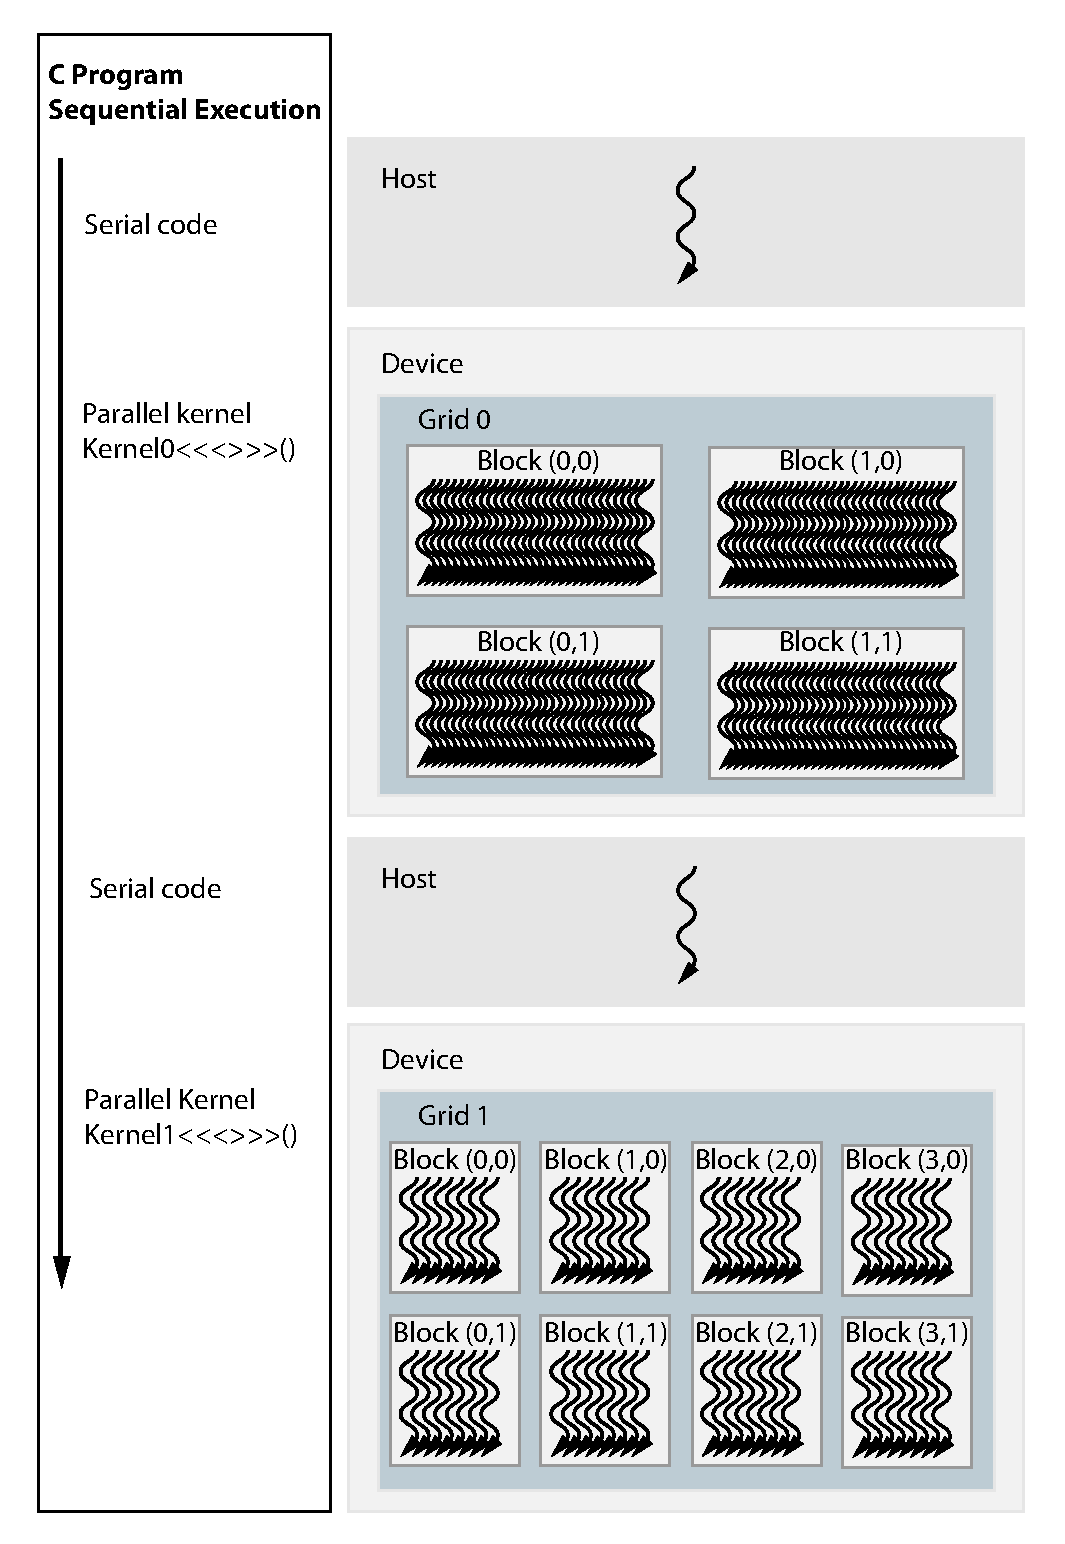
\includegraphics[width=5cm]{../media/cuda_exe.pdf}
%        \end{center}
%    \end{figure}
%  \column{0.5\textwidth}
%Only compute intensive portions of the code which exhibit massive parallelism are computed on the GPU.  The rest of the code runs as traditional sequential C code. 
%\end{columns}
%
%\end{frame}
%
%\section{GPU Memories}
%\begin{frame}{GPU Memories}
%\begin{columns}
%  \column{0.5\textwidth}
%    \begin{figure}[ht]
%    	\begin{center}
%        		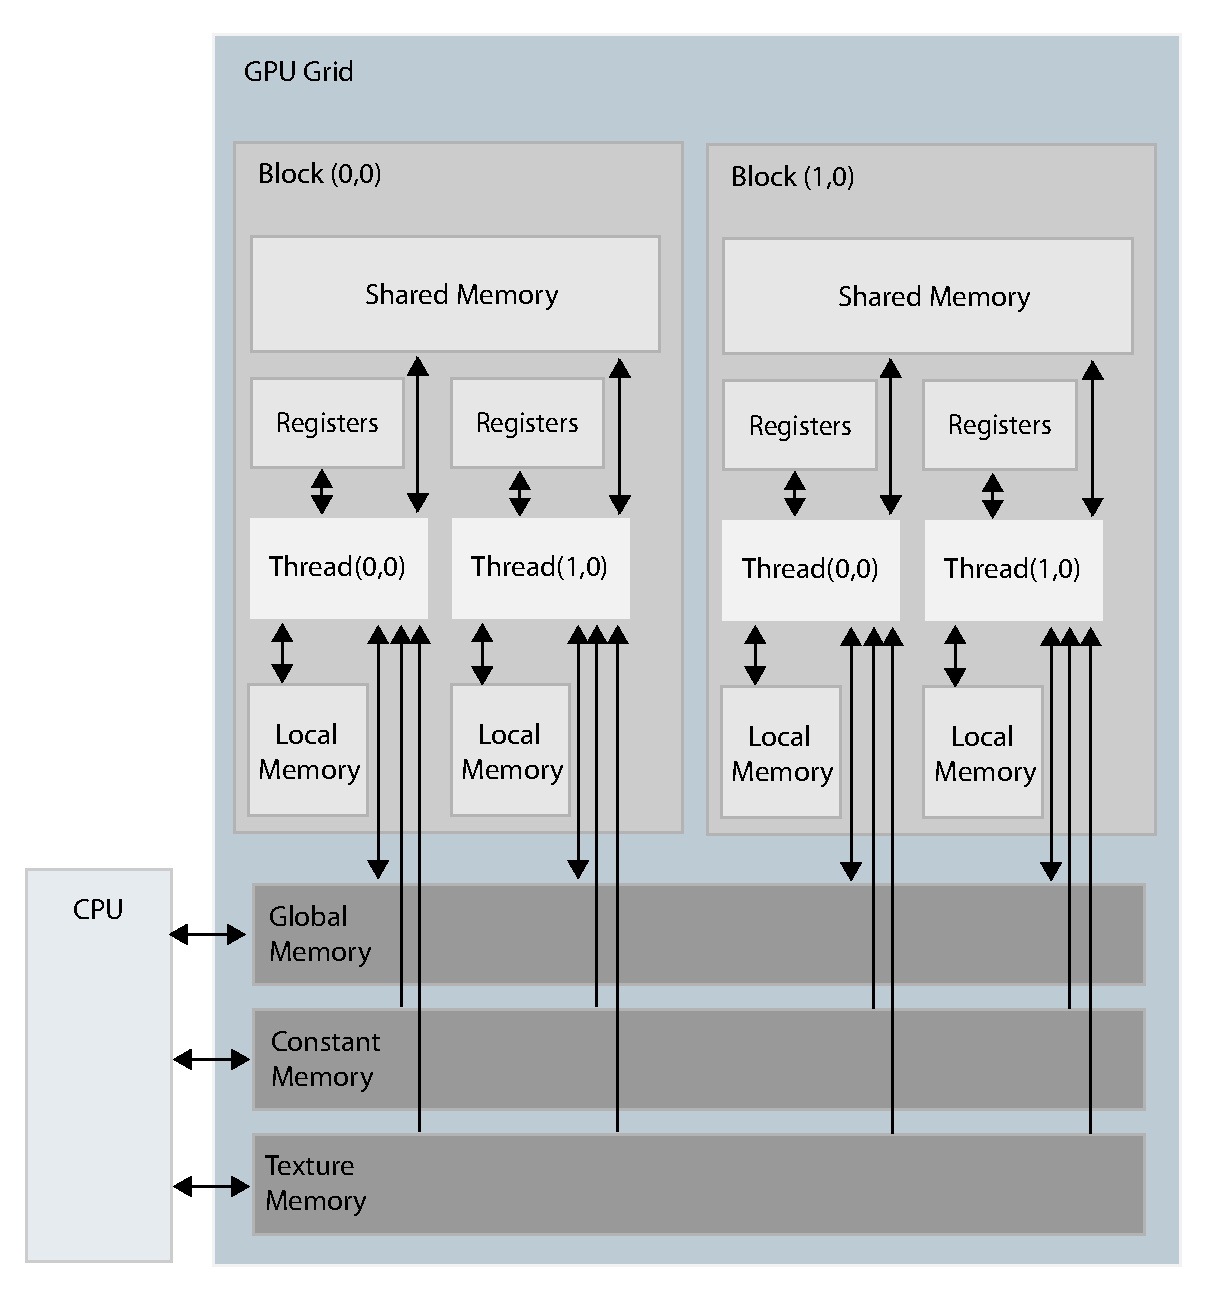
\includegraphics[width=5.5cm]{../media/cuda_mem.pdf}
%        \end{center}
%    \end{figure}
%  \column{0.5\textwidth}
%Only compute intensive portions of the code which exhibit massive parallelism are computed on the GPU.  The rest of the code runs as traditional sequential C code. 
%\end{columns}
%
%\end{frame}


\end{document}
